\documentclass[11pt]{article}

% parameters are fairly self-explanatory here, thankfully
\usepackage[width=7in,height=9.5in,top=0.75in,centering]{geometry}

% for math-ing
\usepackage{amsmath}
\usepackage{amssymb}

%%%%%% tables %%%%%%%%

\usepackage{array}
\renewcommand{\arraystretch}{1.5}
\setlength{\tabcolsep}{8pt}

%%%%%% plotting %%%%%%

\usepackage[dvipsnames]{xcolor}
\usepackage{tikz}
\usepackage{pgfplots}

\pgfplotsset{every axis/.append style={
                    axis x line=middle,    % put the x axis in the middle
                    axis y line=middle,    % put the y axis in the middle
                    axis line style={<->,color=black}, % arrows on the axis
                    xlabel={$x$},          % default put x on x-axis
                    ylabel={$y$},          % default put y on y-axis
            }}
            
 \pgfplotsset{compat=1.14} % sometimes, everything falls apart without this
 
 %\usepgfplotslibrary{fillbetween} %for shading between curves

%%%%%% commands %%%%%%

\def\todo{\textcolor{red}{TODO}}

% exam heading; course name is first argument, exam information is second argument
\newcommand{\Heading}[2]{
    \fbox{
        {\Large\textbf{#1}}
        }
    \hfill
    \fbox{
        \begin{minipage}{0.2\textwidth}
            \begin{center}
            \textbf{#2}
            \end{center}
        \end{minipage}
    }
    \par\vspace{0.1in}}

% for being lazy while beautifying integrals
\newcommand{\dint}{\displaystyle\int}

% for being lazy while beautifying limits
\newcommand{\dlim}{\displaystyle\lim}

%%%%%% stuff %%%%%%

\usepackage{fancyhdr}

%\setcounter{page}{0} % first page is page 0

\parindent0pt % no indent

\fboxsep=0.25cm % little space in fbox border

%%%%%% BEGIN! %%%%%%%

\begin{document}

\pagestyle{fancy}

% record goals here to create sense of transparency

\fancyhead[c]{%
  \ifcase\value{page}
  \or
  \or {\bf\color{RedOrange} A2: Local and Absolute Extreme Values}% page = 5
  \or {\bf\color{RedOrange} A3: Applied Optimization}% page = 7
  \or {\bf\color{Fuchsia} I1: Meaning of an Integral}% page = 3
  \or {\bf\color{Fuchsia} I2: Properties of Definite Integrals}% page = 4
  \or {\bf\color{Fuchsia} I3: Antiderivatives and Indefinite Integrals}% page = 5
  \or {\bf\color{Fuchsia} I4: Compute Definite Integrals}% page = 6
  \or {\bf\color{ProcessBlue} F3: Summations}% page = 7
  \or {\bf\color{Orange} P1: Discrete Random Variables}% page = 8
  \or {\bf\color{Orange} P2: Continuous Random Variables}% page = 9
  \or
  \else
  % Empty chead here!
  \fi
}

% \thispagestyle{empty} % don't display that this is page 0

\Heading{MATH 1210}{Review Session 4\\
A2--A3, I1--I4, F3, P1--P2\\
Spring 2026\\
Section 930}

\vspace{0.1in}

\textbf{Name} \hrulefill

\begin{itemize}
\item\textbf{First Derivative Test.}
Suppose that $c$ is a
\textbf{critical number}
of a continuous function $f$.
\begin{enumerate}
\item
If $f'$ changes from
\textbf{positive}
to
\textbf{negative}
at $c$, then $f$ has a
\textbf{local maximum} at $c$.
\item
If $f'$ changes from
\textbf{negative}
to
\textbf{positive}
at $c$, then $f$ has a
\textbf{local minimum}
at $c$.
\item
If $f'$ does not change sign at $c$,
then $f$ has
\textbf{neither local maximum, nor local minimum}
at $c$.
\end{enumerate}
\vfill
\item\textbf{Second Derivative Test.}
Suppose $f''$ is continuous near a critical number $x=c$.
\begin{enumerate}
\item
If \textbf{$f^{\prime}(c)=0$ and $f^{\prime\prime}(c)<0$}
then we have a
\textbf{local maximum at $x=c$}.
\item
If \textbf{$f^{\prime}(c)=0$ and $f^{\prime\prime}(c)>0$}
then we have a
\textbf{local minimum at $x=c$}.
\item
If \textbf{$f^{\prime}(c)$ DNE,
$f^{\prime\prime}(c)=0$, or
$f^{\prime\prime}(c)$ DNE}
then we cannot use the Second Derivative Test\\
(i.e. the \textbf{test is inconclusive}).
\end{enumerate}
\vfill
\item
\textbf{Closed Interval Method.}
To find the absolute maximum value and absolute minimum value of a continuous function $f$ on the closed interval $[a, b]$, do the following:
\smallskip

\begin{minipage}{0.75\textwidth}
\begin{enumerate}
\item  Find the critical numbers $c_1, c_2, \ldots, c_n$ of $f$ that lie in $(a, b)$.
\item  Find the value of $f$ at each critical number {\em and} at the endpoints


\item  The largest value from (b)  will be the absolute maximum value of $f$ on $[a, b]$ and the smallest value from (b) will be the absolute minimum value of $f$ on $[a, b]$. 
\end{enumerate}
\end{minipage}
%
\hfill
%
\begin{minipage}{0.2\textwidth}
\begin{center}
\begin{tabular}{|c|c|}
\hline 
$x$ & $f(x)$\tabularnewline
\hline 
\hline 
$a$ & $f(a)$\tabularnewline
\hline 
$b$ & $f(b)$\tabularnewline
\hline 
$c_1$ & $f(c_1)$\tabularnewline
\hline 
$c_2$ & $f(c_2)$\tabularnewline
\hline 
$\vdots$ &$\vdots $\tabularnewline
\hline 
$c_n$ & $f(c_n)$\tabularnewline
\hline 
\end{tabular}
\end{center}
\end{minipage}
\vfill
\item
\textbf{First Derivative Test for Absolute Extrema.}
Suppose that $c$ is a critical number of a continuous function $f$ defined on an interval $I$.
    \begin{itemize}
    \item {\bf If} the sign of $f'$ changes from positive ($+$) to negative ($-$) at $c$ {\bf and} $c$ is the only critical number where $f^{\prime}$ changes sign on $I$
    %\emph{and} if $c$ is the only $x$-value in $I$ at which $f$ changes sign, 
    {\bf then} $f(c)$ is the absolute maximum value of $f$ on $I$.
    \item {\bf If} the sign of $f'$ changes from negative ($-$) to positive ($+$) at $c$ {\bf and} $c$ is the only critical number where $f^{\prime}$ changes sign on $I$
    % \emph{and} if $c$ is the only $x$-value in $I$ at which $f$ changes sign, 
    {\bf then} $f(c)$ is the absolute minimum value of $f$ on $I$.\\
    \end{itemize}
\end{itemize}
\newpage

\begin{enumerate}
\item[\textbf{A2.}]
Let $f(x)=\ln|x^2-6x|$
(Note: it is a logarithm of the \emph{absolute value} of $x^2-6x$).
Additionally, note that $f'(x)=\dfrac{2x-6}{x^2-6x}$ and $f''(x)=\dfrac{-2x^2+12x-36}{(x^2-6x)^2}$.
\begin{itemize}
\item[(a)] Find all critical numbers of $f$.
    
    \vfill
    \vfill
    
\item[(b)] For each critical number, determine whether a local maximum, a local minimum, or neither occurs at the critical number.

    \vfill
    \vfill
    \vfill

\item[(c)] Identify the absolute extrema of $f$ on the interval $[1,4]$.

    \vfill
    \vfill

\end{itemize}
\newpage


\item[\textbf{A3.}]
You are building five identical pens adjacent to each other with a
total area of $1000\ \text{m}^2$,
as shown in the following figure.
What dimensions should you use to minimize the amount of fencing?
\begin{center}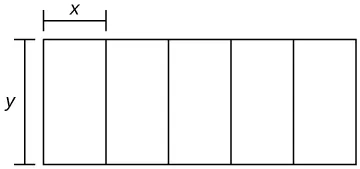
\includegraphics[width=0.4\textwidth]{../../images/pens.png}\end{center}
\newpage


\item[\textbf{I1.}]
You may simply record your answers with no work shown. Please show your work to part (d). ({\bf Note:} Below, ``NOTOA" means ``none of the other answers".)

    \begin{itemize}

    \item[(a)] Suppose $f$ is a continuous function of the variable $x$, $0\leq x\leq 100$. If $f$ is measured in kilograms per cubic meter (kg/m$^3$) and $x$ is measured in square meters (m$^2$), then which of the following are the units of $\displaystyle\int_0^{100} f(x)\,dx$?\\

    \,\hfill
    \fbox{A} kg$\cdot$m
    \hfill
    \fbox{B} kg/m$^3$
    \hfill
    \fbox{C} kg/m$^2$
    \hfill
    \fbox{D} kg/m
    \hfill
    \fbox{E} NOTOA
    \hfill\,\\

    \item[(b)] If $h(t)$ represents the heart rate (in beats per minute) of a sprinter $t$ minutes after starting a 400-meter dash, then what does $\displaystyle\int_0^{1} h(t)\,dt$ represent in this context?
    \vfill

    \item[(c)] Let $h(t)$ represent the heart rate (in beats per minute) of a sprinter $t$ seconds after starting a race. Assume the sprinter's heart rate increases faster and faster as the race progresses. Consider the quantities below.\\[0.2in]
    %
    \,\hfill
    I: $\displaystyle\int_{0}^{0.4} h(t)\,dt$
    \hfill
    II: $\displaystyle\int_{0}^{0.6} h(t)\,dt$
    \hfill
    III: $\displaystyle\int_{0.4}^{1} h(t)\,dt$
    \hfill
    IV: $\displaystyle\int_{0.6}^{1} h(t)\,dt$
    \hfill\,\\

    With the given information, which of the following {\it could} correctly order these quantities from least to greatest? Circle all possibilities.\\[0.2in]
    %
    \,\hfill
    \fbox{A} $I<II<IV<III$
    \hfill
    \fbox{B} $I<III<IV<II$
    \hfill
    \fbox{C} $II<I<IV<III$
    \hfill\,\\
    
    \,\hfill
    \fbox{D} $IV<III<I<II$
    \hfill
    \fbox{E} $III<IV<II<I$
    \hfill\,\\

    \item[(d)] Let $T'(t)$ represent the (instantaneous) rate of change (in $^{\circ}$C/hour) of temperature in Charlottesville at a time $t$ (in hours) during a particular day. Assume the temperature at midnight was $0^{\circ}$C, and the temperature at 10:00 AM was $5^{\circ}$C. Which of the following expressions must represent the temperature at noon? Circle all correct answers.\\[0.2in]
    %
    \,\hfill
    \fbox{A} $5+\displaystyle\int_{10}^{12} T'(x)\,dx$
    \hfill
    \fbox{B} $5-\displaystyle\int_{10}^{12} T'(x)\,dx$
    \hfill
    \fbox{C} $\displaystyle\int_{10}^{12} T'(x)\,dx-5$
    \hfill\,\\
    
    \,\hfill
    \fbox{D} $5+\displaystyle\int_0^{12} T'(x)\,dx$
    \hfill
    \fbox{E} $5-\displaystyle\int_0^{12} T'(x)\,dx$
    \hfill
    \fbox{F} $\displaystyle\int_0^{12} T'(x)\,dx$
    \hfill
    \fbox{G} NOTOA
    \hfill\,\\
    \end{itemize}
\newpage


\item[\textbf{I2.}]
The graph of the function $f$ consists of a semicircle followed by two line segments, and is given below:

\begin{center}
    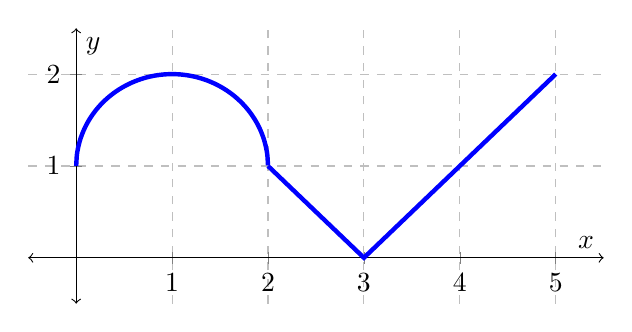
\begin{tikzpicture}
          \begin{axis}[
        %    axis y line = left,
        %    axis x line = bottom,
            xlabel = {$x$},
            ylabel = {$y$},
            ytick       = {1,2,3,4,5},
            yticklabels = {1,2,3,4,5},
            xtick       = {1,2,3,4,5},
            xticklabels = {1,2,3,4,5},
            samples     = 320,
            %domain      = 0:4,
            %restrict y to domain=-5:5,
            ymin = -0.5, ymax = 2.5,
            xmin = -0.5, xmax = 5.5,
            width=3.5in,height=2in,
            grid=both, grid style=dashed
          ]
         %
         \addplot[domain=0:2,blue, ultra thick, mark=none, smooth] {1+(1-(x-1)^2)^(1/2)};
         \draw[ultra thick,blue] (2,1) -- (3,0) -- (5,2);
         %
         \end{axis}
    \end{tikzpicture}    
\end{center}

\begin{itemize}

% \item[(a)] Estimate $\displaystyle\int_0^5 f(x)\,dx$ using $L_5$. Sketch your estimate above.
%     \vfill
    
\item[(a)] Find the exact value of $\displaystyle\int_0^5 f(x)\,dx$.
    \vfill
    
\item[(b)] Suppose for some function $g$ that $\displaystyle\int_0^5 (2f(x)-3g(x))\,dx=\pi$. Find $\displaystyle\int_0^5 g(x)\,dx$.
    \vfill
    
\end{itemize}
\newpage

\item[\textbf{I3.}]
Write down the indefinite integrals of the following expressions. 

Although no work is required, you are encouraged to include any work that shows your thought process. 

%constant, power, exponential, log, +C, algebraic manipulation

\begin{center}
        \begin{tabular}{l c r l c r}
            $\displaystyle\int x^{-12}\,dx$ & $=$ & \rule[-8pt]{1.5in}{0.4pt} &
            $\displaystyle\int e^{14} \,dx$ & $=$ & \rule[-8pt]{1.5in}{0.4pt}\\[1in]
            $\displaystyle\int e^x\,dx$ & $=$ & \rule[-8pt]{1.5in}{0.4pt}&
            $\displaystyle\int 3e^x+x^{90}\,dx$ & $=$ & \rule[-8pt]{1.5in}{0.4pt}\\[1in]
            $\displaystyle\int \frac{17}{x} \,dx$ & $=$ & \rule[-8pt]{1.5in}{0.4pt} & 
            $\displaystyle\int \dfrac{17}{x^2} \,dx$ & $=$ & \rule[-8pt]{1.5in}{0.4pt}\\[1in]
            $\displaystyle\int 12^2 \ln(12)\,dx$ & $=$ & \rule[-8pt]{1.5in}{0.4pt} &
            $\displaystyle\int 12^x \ln(12) \,dx$ & $=$ & \rule[-8pt]{1.5in}{0.4pt}\\[1in]
        \end{tabular}
\end{center}
\newpage

\item[\textbf{I4.}]
Respond to the following prompts regarding definite integrals.
\item[(a)] On which of the following integrals could the Fundamental Theorem of Calculus be used? Circle all correct answers
and compute all the integrals on which the Fundamental Theorem of Calculus can be used. ({\bf Note:} Below, ``NOTOA" means ``none of the other answers".)

\

\,\hfill
\fbox{A} $\displaystyle\int_{-1}^2 \sqrt{x}\,dx$
\hfill
\fbox{B} $\displaystyle\int_{1}^3 \frac{x+3}{x^2}\,dx$
\hfill
\fbox{C} $\displaystyle\int_{2}^{-4} 2^x \ln(2)\,dx$
\hfill
\fbox{D} $\displaystyle\int_0^{\pi/4} \frac{1}{x}\,dx$
\hfill
\fbox{E} NOTOA
\hfill\,

\vfill

\item[(b)] Compute $\displaystyle\int_{1}^{e}\left( x+\frac1x\right)\,dx$. You do not have to simplify your final answer.
\vfill
\newpage

\item[\textbf{F3.}]
Respond to the following prompts regarding summations.
\begin{enumerate}
\item[(a)] Expand the following summation completely. You may simply write your answer. Do not simplify your answer.\\

\[\sum_{n=1}^{5} \frac{2^n}{n^2+1} = \rule[-10pt]{5.25in}{0.4pt} \]

    \vfill

\item[(b)] Fill in the blank to write the following sum using summation notation. You may simply write your answer.\\

{%\Large
\[-2 + 1 - \frac{1}{2} + \frac{1}{4} - \frac{1}{8} = \rule[-10pt]{5in}{0.4pt}\]
}

    \vfill

\item[(c)] Use properties of summations exhaustively (that is, until they can't be used any more) to rewrite the following summation. You may simply write your answer.\\

{%\Large
\[ \sum_{n=1}^{100}\left(\frac{a_n}{b_n} - 2c_n\sqrt{d_n} - \frac{1}{100} \right) = \rule[-10pt]{4in}{0.4pt}\]
}

    \vfill

\end{enumerate}
\newpage

\item[\textbf{P1.}]
A bag contains 2 blue marbles, 1 red marble, and 1 yellow marble.
A marble is drawn, its color recorded, and then returned to the bag.
This process is repeated \textbf{once more}.

\begin{enumerate}
\item
What is the sample space $S$?
{\Large
\[
S = \rule[-8pt]{4in}{0.4pt}
\]
}

\item
Let $X$ be a random variable equal to the
number of times a blue marble is drawn,
and let $p(x)$ be its probability mass function.
Fill out the table of values of $p(x)$.

\vspace{0.5cm}

\begin{minipage}{0.45\textwidth}
\centering    
\begin{tabular}{|c|ccc|}
    \hline
   $x$  & & &  \\
   \hline
   $p(x)$  & & \hphantom{123123123} &\\
   \hline
\end{tabular}
\end{minipage}
\vspace{.5in}
\item
Compute the probability that $X$ is even.
\vfill

\item
\begin{itemize}
\item Compute $E[X]$.
\vfill
\item Compute $E[X^2]$.
\vfill
\item Compute $Var(X)$.
\vfill
\end{itemize}
\end{enumerate}
\newpage

\item[\textbf{P2.}]
Let $X$ be a continuous random variable. The following graph is either the graph of the PDF $p(x)$ or the CDF $C(x)$.
The function is defined by the formula on the right.

\begin{center}
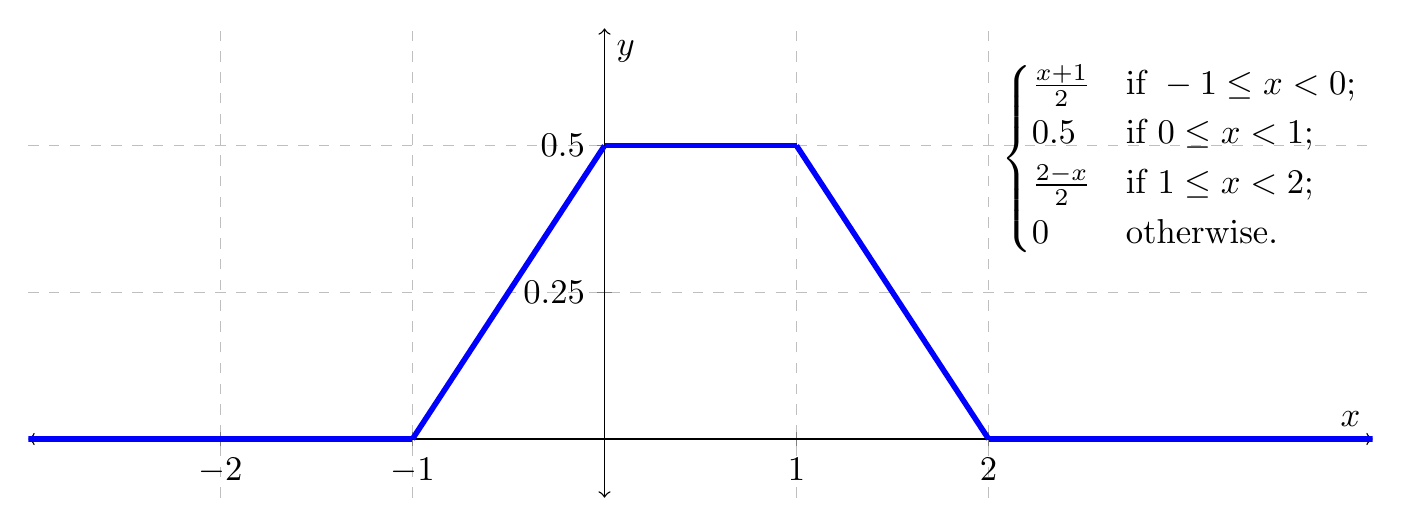
\begin{tikzpicture}[scale=1.25]
\begin{axis}[
 xlabel={$x$},
 %grid = major,
 xtick       = {-2,-1,0,1,2},
 xticklabels = {$-2$,$-1$,$0$,$1$,$2$},
 ytick       = {0, 0.25, 0.5},
 yticklabels = {$0$, $0.25$, $0.5$},
 samples     = 320,
 domain      = -3:5,
 restrict y to domain=-3.5:2.5,
 xmin = -3, xmax = 4,
 ymin = -0.1, ymax = 0.7,
 height=2.5in, width=6in,
 grid=both, grid style=dashed
]
\draw[ultra thick, blue,-] (-4,0)--(-1,0);
\draw[ultra thick, blue,-] (-1,0)--(0,0.5);
\draw[ultra thick, blue,-] (0,0.5)--(1,0.5);
\draw[ultra thick, blue,-] (1,0.5)--(2,0);
\draw[ultra thick, blue,-] (2,0)--(4,0);
\coordinate[label={$\begin{cases}
    \frac{x+1}{2}& \text{if } -1\leq x< 0;\\
    0.5& \text{if } 0\leq x< 1;\\
    \frac{2-x}{2}& \text{if } 1\leq x< 2;\\
    0& \text{otherwise}.
\end{cases}$}, yshift=-0.5in] (A) at (3,0.5);
\end{axis}
 \end{tikzpicture}
     \end{center}

\begin{enumerate}
    \item[(a)] Determine whether the graph is of $p(x)$ or $C(x)$, and explain why. 

    \vfill

    \item[(b)] Based on the graph, what is the probability that the value of $X$ falls between $\frac{-1}{2}$ and $\frac{1}{2}$?

    \vfill

    \item[(c)] What is the support of $X$?

    \vfill

    \item[(d)] Find the formula or the graph of the PDF $p(x)$ or the CDF $C(x)$, which ever is NOT represented by the given graph.

    \vfill
\end{enumerate}
\newpage

\end{enumerate}
\end{document}